\documentclass[aspectratio=169,xcolor=dvipsnames]{beamer}

% Cambridge house-style theme (dropped in under theme/). TEXINPUTS in the
% Makefile adds theme/ to the search path so \usetheme{cambridge} resolves.
\usetheme{cambridge}

\usepackage[utf8]{inputenc}
\usepackage[T1]{fontenc}
\usepackage{lmodern}
\usepackage{amsmath,amssymb,bm}
\usepackage{booktabs}
\usepackage{tikz}
\usepackage{tensor}
\usetikzlibrary{arrows.meta,positioning,shapes.geometric,decorations.pathmorphing,
                fadings,decorations.markings,calc}
\usepackage{graphicx}
\graphicspath{{figures/}}
% standalone: allows \input{figures/*.tex} to work (strips outer \documentclass)
\usepackage{standalone}

% \todo{...} placeholder boxes for unfinished content.
\usepackage[colorinlistoftodos,textsize=scriptsize]{todonotes}
\newcommand{\placeholder}[1]{\todo[inline,color=yellow!40]{#1}}

% Macros matching research/lagrangian_enumeration/general_quadratic_lagrangian.tex
\newcommand{\Rt}{\tilde{R}}
\newcommand{\Mpl}{M_{\mathrm{pl}}}
\newcommand{\eps}{\varepsilon}
\newcommand{\del}{\partial}

\setbeamertemplate{frame numbering}[fraction]
\setbeamertemplate{navigation symbols}{}

% Cambridge theme's enumerate item template uses \insertenumlabel which
% is recursive with current beamer; override with \arabic-based numbering.
\setbeamertemplate{enumerate item}{\arabic{enumi}.}
\setbeamertemplate{enumerate subitem}{\arabic{enumi}.\arabic{enumii}}
\setbeamertemplate{enumerate subsubitem}{\arabic{enumi}.\arabic{enumii}.\arabic{enumiii}}

% ---- Metadata ---------------------------------------------------------------
\title[Graviton-photon conversion in PGT]%
      {Graviton-Photon Conversion in Poincar\'e Gauge Theory}
\subtitle{A phenomenological survey}
\author{William Royce}
\institute{Cavendish Astrophysics \\ University of Cambridge}
\date{Practice talk --- \today}

% ---- Main deck --------------------------------------------------------------
\begin{document}

\begin{frame}[plain]
  \titlepage
\end{frame}

\begin{frame}{Why this talk}
  \note{\textasciitilde 1 min mark. Set the stakes, promise a clear question, promise the tool.}
  \begin{itemize}
    \item Gravitational waves are now a routine observable --- the next frontier is \emph{high-frequency} and \emph{beyond-GR} couplings.
    \item Any channel linking gravity and electromagnetism \emph{at linear order} is a candidate probe of new physics.
    \item This talk:
      \begin{enumerate}
        \item one such channel --- the Gertsenshtein effect;
        \item one beyond-GR question --- does \emph{torsion} modify it?;
        \item one tool built to answer it systematically --- \textsc{tidal}.
      \end{enumerate}
  \end{itemize}
\end{frame}

\begin{frame}{Graviton--photon conversion}
  \textbf{Setup:} Linearised GR $+$ Maxwell $+$ uniform background $B$.

  \vspace{0.3em}
  \textbf{Why they mix:} EM action $-\frac{1}{4} F_{\mu\nu} F^{\mu\nu}$ has \textcolor{Cambridge24DarkCrest}{two metric factors} AND two EM field strengths.  Linearise $g = \eta + \textcolor{Cambridge24DarkCrest}{h}$ and $F = \textcolor{Cambridge24Cherry}{\bar F} + \textcolor{Cambridge24Indigo}{\delta F}$:
  \[
    S_{\rm EM} \propto \int (\eta + \textcolor{Cambridge24DarkCrest}{h})(\eta + \textcolor{Cambridge24DarkCrest}{h})\,(\textcolor{Cambridge24Cherry}{\bar F} + \textcolor{Cambridge24Indigo}{\delta F})(\textcolor{Cambridge24Cherry}{\bar F} + \textcolor{Cambridge24Indigo}{\delta F})
  \]
  Pick \emph{one $\textcolor{Cambridge24DarkCrest}{h}$, one $\textcolor{Cambridge24Indigo}{\delta F}$, one $\textcolor{Cambridge24Cherry}{\bar F}$}: a direct $h \leftrightarrow \gamma$ coupling $\propto \textcolor{Cambridge24Cherry}{\bar F} = B$.

  \vspace{0.3em}
  \begin{center}
    \colorbox{CambridgeLight}{%
      \begin{minipage}{0.7\linewidth}
        \vspace{0.4em}\centering
        {\Large $\displaystyle P_{g\to\gamma}(L) = \sin^{2}\! \left(\tfrac{1}{2}\kappa B L\right)$}
        \vspace{0.4em}
      \end{minipage}}
  \end{center}
  \vspace{0.3em}
  Two-state mixing; off-diagonal coupling $B$.  At magnetar $B\sim 10^{11}$\,T over $L\sim 10^{6}$\,km: $P\sim 10^{-8}$.

\end{frame}

\begin{frame}{Why the weakness is fundamental}
  \note{\textasciitilde 4 min mark. Planck-scale suppression is structural. Classic literature establishes this. Then bridge: the only way out is new physics.}
  \textbf{Planck-scale suppression:}
  \[
    P \;\sim\; \left(\frac{B_0 D}{M_{\rm Pl}}\right)^{\!2}, \qquad M_{\rm Pl}\sim 10^{19}\,\text{GeV}
  \]
  Even for a magnetar ($B_0\sim 10^{15}$\,G over $\sim\!10$\,km), $B_0 D / M_{\rm Pl} \sim 10^{-5}$, giving $P\sim 10^{-10}$. This is a structural consequence of the Planck scale --- not an engineering limit.

  \vspace{0.15em}
  \textbf{What the literature established:}
  \begin{itemize}\small
    \item \textbf{Gertsenshtein 1962} --- original effect; conversion immediately recognised as hopelessly small.
    \item \textbf{Boccaletti et al.\ 1970} --- full analytic solution for a localised $B$-field region.
    \item \textbf{Raffelt \& Stodolsky 1988} --- embedded in the axion--photon mixing context; the paper modern work cites.
  \end{itemize}

  \vspace{0.15em}
  \emph{The formula is exact in linearised Einstein--Maxwell. The weakness is the Planck scale --- not a calculation gap. Any amplification requires new gravitational physics.}
\end{frame}

\begin{frame}{Torsion via Poincar\'e gauging}

  \textbf{Spacetime has two independent local symmetries.}
  Local Lorentz and coordinate freedoms are \emph{gauge redundancies} of the Poincar\'e group --- motivating a gauge treatment of gravity.
  \begin{center}
    \begin{tabular}{lll}
      \toprule
      Gauge group & Connection & Field strength \\
      \midrule
      (QED) &$U(1)$                  & $A_\mu$             & $\mathcal{F}_{\mu\nu}$ \\
      (Lorentz) &$SO(1,3)$           & $\omega^{ab}{}_\mu$ & \textbf{curvature} $\mathcal{R}^{ab}{}_{\mu\nu}$ \\
      (Translations) &$\mathbb{R}^4$ & $e^a{}_\mu$         & \textbf{torsion}   $\mathcal{T}^a{}_{\mu\nu}$ \\
      \bottomrule
    \end{tabular}
  \end{center}

  \vspace{0.25em}
  GR ($V_4$): $\mathcal{R}\neq 0$, $\mathcal{T}=0$, $\mathcal{Q}=0$.\quad
        PGT ($U_4$): $\mathcal{R}\neq 0$, $\mathcal{T}\neq 0$, $\mathcal{Q}=0$.\quad
        Torsion is the new degree of freedom.
\end{frame}

\begin{frame}{The systematic landscape}
  \begin{columns}[T,onlytextwidth]
    \begin{column}{0.44\textwidth}
      Don't pick a theory --- scan the full quadratic landscape:
      \vspace{-0.3em}
      \[
        \mathcal{L} \supset
          \underbrace{\alpha_i I_i}_{T^2}
          +
          \underbrace{\beta_i \Rt^2_{(i)}}_{\Rt^2}
          +
          \underbrace{\delta_1 \Rt_{[\mu\nu]}F^{\mu\nu}+\cdots}_{\text{non-min.}}
          -\tfrac{1}{4}F^2
      \]
      \vspace{-0.4em}
      {\scriptsize\setlength{\itemsep}{-2pt}
      \begin{itemize}
        \item \textbf{$T^2$ (3):} torsion kinetics --- tensor, axial, vector irreps propagate independently
        \item \textbf{$\Rt^2$ (6):} graviton self-coupling; propagating torsion enters
        \item \textbf{Non-minimal:} geometry--EM vertex absent in GR --- primary target for enhanced conversion
      \end{itemize}}
    \end{column}
    \begin{column}{0.53\textwidth}
      {\renewcommand{\arraystretch}{0.52}
      \begin{center}\tiny
        \begin{tabular}{@{}lllc@{}}
          \toprule
          \textbf{Sector} & \textbf{Parameters} & \textbf{Lit.} & \textbf{N} \\
          \midrule
          $\Rt^2$ & $\alpha_1\ldots\alpha_6$ & B: $\alpha_{1\text{--}6}$ & 6 \\
          $T^2$ & $\beta_1,\beta_2,\beta_3$ & B: $\beta_{1\text{--}3}$; S: $I_{1\text{--}3}$ & 3 \\
          $F^2$ & $\gamma_1$ & --- & 1 \\
          $\Rt\times F$ & $\delta_1$ & --- & 1 \\
          \midrule
          $\eps\cdot\Rt^2$ & $d_1\ldots d_{13}$ & --- & 13 \\
          $\eps\cdot T^2$ & $d_{14}\ldots d_{17}$ & --- & 4 \\
          $\eps\cdot F^2$ & $d_{18}$ (topo) & --- & 1 \\
          $\eps\cdot\Rt\times F$ & $d_{19},d_{20},d_{21}$ & --- & 3 \\
          \midrule
          $\del T\times F$ & $\zeta_1,\zeta_2,\zeta_3$ & S: $\theta_{2,5,6}$ & 3 \\
          $\Rt\times\del T$ & $\chi,\chi_2\ldots\chi_{10}$ & B: $\chi$ & $10$ \\
          $(\del T)^2$ & $\xi,\xi_2\ldots\xi_{16}$ & B: $\xi$ & $16$ \\
          \midrule
          $\eps\cdot\del T\times F$ & $\tilde{\zeta}_{1\text{--}6}$ & --- & 6 \\
          $\eps\cdot\Rt\times\del T$ & $\tilde{\chi}_{1\text{--}36}$ & --- & $36$ \\
          $\eps\cdot(\del T)^2$ & $\tilde{\xi}_{1\text{--}38}$ & --- & $38$ \\
          \bottomrule
        \end{tabular}
      \end{center}}
    \end{column}
  \end{columns}
\end{frame}

\begin{frame}{The question}
  \note{\textasciitilde 7.5 min mark. Sharpest possible framing, then pivot to the tool.}
  \begin{block}{}
    \centering
    \emph{In a PGT $+$ Einstein--Maxwell Lagrangian,\\
    does torsion modify the Gertsenshtein conversion probability,\\
    and if so, through which coupling and in which regime?}
  \end{block}
  \vspace{0.5em}
  \textbf{Sub-question:} \emph{what does the Lagrangian have to look like} for torsion to matter at all?
  \vspace{0.8em}

  To answer that at the level of an \emph{arbitrary} Lagrangian --- and to do it often enough to sweep parameter space --- I built \textsc{tidal}.
\end{frame}

\begin{frame}{\textsc{tidal}: overview}
  \begin{tikzpicture}[overlay,remember picture]
    \node[anchor=north east,inner sep=0pt,xshift=-0.45cm,yshift=-0.32cm]
      at (current page.north east)
      {
\includegraphics[height=1.0cm]{TIDAL_Logo_TikZ_Figure}};
  \end{tikzpicture}%
  \vphantom{.}{\large \textbf{T}}ensor {\large \textbf{I}}ntegration and {\large \textbf{D}}erivation for {\large \textbf{A}}ny {\large \textbf{L}}agrangian.

  \vspace{0.3em}
  \begin{center}
    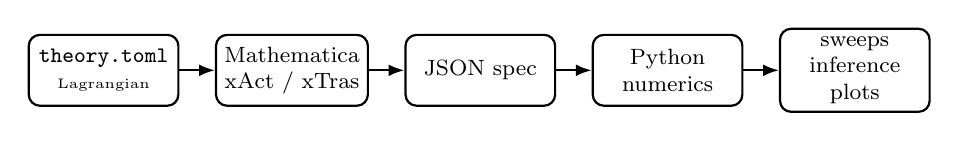
\begin{tikzpicture}[
      node distance=0.5cm and 0.45cm,
      every node/.style={font=\footnotesize},
      box/.style={draw,rounded corners,thick,align=center,
                  minimum height=0.9cm,minimum width=1.9cm,inner sep=3pt},
      arr/.style={-{Latex[length=2mm]},thick},
    ]
      \node[box] (toml)   {\texttt{theory.toml}\\\tiny Lagrangian};
      \node[box,right=of toml]   (wolf) {Mathematica\\xAct / xTras};
      \node[box,right=of wolf]   (json) {JSON spec};
      \node[box,right=of json]   (num)  {Python\\numerics};
      \node[box,right=of num]    (out)  {sweeps\\inference\\plots};
      \draw[arr] (toml)--(wolf);
      \draw[arr] (wolf)--(json);
      \draw[arr] (json)--(num);
      \draw[arr] (num)--(out);
    \end{tikzpicture}
  \end{center}

  \vspace{0.2em}
  \emph{Every equation in the numerical solver is derived
  symbolically from a single Lagrangian declaration.} Automatic Euler--Lagrange variation, multi-field perturbation, and the covariant-derivative expansion.

  \vspace{0.2em}
  PGT surveys vary the Lagrangian
  across dozens of operator combinations. At this level of generality, the associated tensor calculus become intractable by hand
  --- symbolic computation is the only viable route.

\end{frame}

\begin{frame}{Modal solver}
  A spectral solver for the linearised gauge theories the survey
  produces. Two regimes --- per-mode (uniform $B_0$) and convolution-coupling (localised $B_0(x)$) --- both evolve by direct matrix
  exponential, \emph{no eigendecomposition}.

  \vspace{0.25em}
  \begin{itemize}\footnotesize
    \item Every theory linearises to periodic, time-independent PDEs around flat backgrounds
    \item Both uniform and localised $B_0$ stay inside the regime (per-mode vs.\ convolution coupling)
    \item Machine-precision time evolution; no time-stepping error
      \end{itemize}

  Off-the-shelf $V\,\mathrm{diag}(e^{\lambda t})\,V^{-1}$ fails universally on gauge theories.
  \begin{itemize}\footnotesize
    \item \textbf{Direct matrix exponential} (Pad\'e / Krylov),
          not eigendecomposition, $V$ catastrophically ill-conditioned
    \item \textbf{Fourier-space algebraic elimination} of fields
          without time derivatives
      \end{itemize}

\end{frame}

\begin{frame}{Nested sampling: surveying the amplification landscape}
  For each $\theta$ we simulate and compute the \emph{amplification factor} relative to the GR baseline:

  \vspace{-0.8em}
  {\Large\[
    A(\theta) = P_{\text{final}}(\theta) \Big/ \sin^2\! \left(\tfrac{\kappa B_0 t}{2}\right)
  \]}
  The score function, the \emph{likelihood}, is $L(\theta) = \pm \log A(\theta)$.
  
  \begin{itemize}
    \item $\mathcal{Z} = \int A(\theta)\,\pi(\theta)\,\mathrm{d}\theta = \langle A\rangle_\pi$ ---
      \textbf{prior-averaged amplification}.
      \begin{itemize}
        \item $\log\mathcal{Z}\approx 0$: null (no enhancement on average);
        \item $\log\mathcal{Z} \gg 0$: theory generically amplifies.
      \end{itemize}     

    \item $D_{\mathrm{KL}} \bigl(p(\theta\,|\,A)\,\Vert\,\pi(\theta)\bigr)$ --- \textbf{information gain}.
    \begin{itemize}
      \item Is enhancement broadly distributed (\emph{generic});
      \item or concentrated in a narrow coupling region (\emph{fine-tuned}).
    \end{itemize}
      

  \end{itemize}
\end{frame}

\begin{frame}{Three results from the scan}
  \begin{enumerate}
    \item \textbf{Minimal PGT (Einstein--Cartan + $I_i + \Rt^2$).}
    \begin{itemize}
      \item The Gertsenshtein channel contains \emph{no torsion fields} coupling.
    \end{itemize}

    \item \textbf{Plasma (Einstein--Maxwell + $m_A^2$).}
    \begin{itemize}
      \item Effective photon mass detunes the resonance: $P_{\max}$ monotonically suppressed by $m_A^2$.
    \end{itemize}

    \item \textbf{Dark-photon} $\mathcal{L} = \frac{1}{\kappa^2} R - \tfrac{1}{4}F^2 - \tfrac{1}{4}\xi F_T^2 + \delta_m F\cdot F_T - \alpha_3 I_3$.
    \begin{itemize}
      \item Torsion as a hidden BSM vector with mass.
      \item No \emph{Vacuum} conversion channel;
      \item \emph{Plasma} effective photon mass adds coupling;
      \item \emph{Negligible} effect: plasma dominates only as suppression again.
    \end{itemize}
  \end{enumerate}
  
\end{frame}

\begin{frame}{Survey progress: what's mapped, what's next}
  \note{\textasciitilde 14 min mark. Show the campaign as a real, partially-executed survey, not an aspiration.}
  \textbf{Stages completed:}
  {\renewcommand{\arraystretch}{0.82}
  \begin{center}\scriptsize
    \begin{tabular}{lll}
      \toprule
      Stage & Theory class & Outcome \\
      \midrule
      A    & Dark-photon plasma           & amplify NULL; \textbf{suppress informative} ($\sim\!100\times$) \\
      B    & Einstein--Cartan             & NULL --- torsion-trace alone is Gertsenshtein-neutral \\
      C    & $R^2$-PGT structural         & algebraic null in TT channel (no run needed) \\
      D1   & Ricci-EM ($\delta_1 R_{[\mu\nu]}F^{\mu\nu}$) & \textbf{strong suppression: BF $\sim\!10^7$} \\
      D2.0 & Bahamonde YM-PGT (5D)        & NULL both directions \\
      D2.1 & Barker $\chi$-axial (6D)     & NULL both directions; $\langle\chi\rangle \approx 0$ \\
      \bottomrule
    \end{tabular}
  \end{center}}

  \vspace{0.2em}
  \textbf{The story so far:} amplification is \emph{elusive}. Multiple PGT extensions are Gertsenshtein-neutral; non-minimal Ricci-EM gives strong \emph{suppression} at $|\delta_1|\!\approx\!1.3$.

  \vspace{0.15em}
  \textbf{Queued / planned:}
  \begin{itemize}\scriptsize
    \item \textbf{D2.2 Shapiro PGT}, \textbf{D2.3 complete-PGT}, \textbf{D3 parity-odd YM-PGT-CP} --- pending derivation.
    \item \textbf{Plasma-Proca extensions} --- effective photon mass; magnetar / IGM observability.
    \item \textbf{T7 Complete-Even-PGT} ($\sim\!10$ couplings), \textbf{T8 Complete-Odd-PGT} ($\sim\!60$) --- gated on D3 finding signal.
  \end{itemize}
  \emph{Each new theory is a config-file change in the pipeline, not a rewrite.}
\end{frame}

\begin{frame}{Summary}
  \begin{itemize}
    \item Bare GR Gertsenshtein: undetectable.  Beyond-GR gravity may amplify.
    \item Built \textsc{tidal} (symbolic derivation $\to$ modal solver $\to$ Bayesian survey); surveyed the PGT operator space.
    \item Amplification and suppression both present at linear order, ghost-free.  Curvature $\times$ torsion-derivative coupling $\Rt\!\cdot\!\nabla\mathcal{T}$ robustly dominant.
    \item Next: localised geometry; PSALTer particle-spectrum analysis.
  \end{itemize}

  \vspace{0.4em}
  \centering Thanks --- questions welcome.
\end{frame}


% ---- Backup slides ---------------------------------------------------------
\appendix
% Backup slides --- shown only in Q&A.

\begin{frame}[plain]
  \centering\Huge Appendices
\end{frame}

\begin{frame}{Magnetar context}
  \centering
  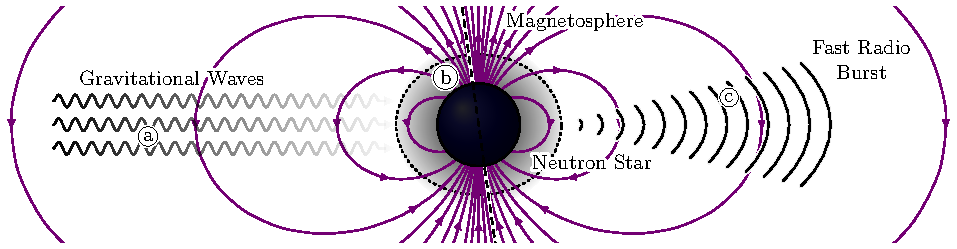
\includegraphics[width=0.8\linewidth]{gertsenshtein_zeldovich_star}
  \vspace{0.4em}

  Magnetar field $B\sim 10^{15}$\,G, scale $\sim 10$\,km: $P_{g\to\gamma}\sim 10^{-10}$.
\end{frame}

\begin{frame}{Full PGT $+$ EM Lagrangian}
  \placeholder{Full Lagrangian with each term labelled in English: Einstein-Cartan, torsion kinetics, curvature-squared, Maxwell, non-minimal couplings.}
\end{frame}

\begin{frame}{Higher-derivative terms: $\Rt^2$ \& $F^4$ via perturbative reduction}
  \scriptsize
  \textbf{Problem.} $\Rt^2$ (and Euler--Heisenberg $(F^2)^2$) produce 4th-order time
  derivatives in the EOMs --- generically Ostrogradsky-ghost modes.  Cannot integrate
  the full theory directly.

  \vspace{0.4em}
  \textbf{Parker--Simon iterative reduction (1993).}  Treat $b_5$ as small;
  the full EOM splits as $E_{\rm base}[y] + b_5\,E_{\rm corr}[y]=0$, where
  $E_{\rm corr}$ contains the 4th-order $\Rt^2$ pieces.  Expand
  $y(k,t) = y^{(0)} + b_5\,y^{(1)} + \cdots$ and collect by order:
  \[
    E_{\rm base}\bigl[y^{(0)}\bigr] = 0,\qquad
    E_{\rm base}\bigl[y^{(n)}\bigr] = -E_{\rm corr}\bigl[y^{(n-1)}\bigr],
    \quad n\ge 1.
  \]
  \emph{The 4th-order operator never acts on the unknown.}  $E_{\rm corr}$ evaluates
  on the previous order's known trajectory, becoming a time-dependent source for the
  next order.  The 4th-order operator is never integrated; ghost eigenvalues never enter the
  propagator.

  The sourced equation is solved analytically by \emph{Duhamel's principle}: convolve
  the base propagator $e^{A(t-\tau)}$ against the source, evaluated analytically in
  the order-$0$ eigenbasis, no numerical quadrature.

  \vspace{0.4em}
  \textbf{Constraint-promotion barrier.}
  At $b_5=0$ (Einstein--Cartan), some metric components are \emph{pure algebraic
  constraints}: non-dynamical, carrying no degrees of freedom.  The $\Rt^2$ correction
  promotes them to propagating fields --- the number of propagating modes
  jumps discontinuously as $b_5\to 0$. No published perturbative Hamiltonian recipe handles
  this case; energy measurements break down across $b_5=0$.
\end{frame}

\begin{frame}{\textsc{tidal} architecture deep-dive}
  \placeholder{CoefficientEvaluator cache levels, operator library, constraint-IC solver, RHS evaluator, state layout.}
\end{frame}

\begin{frame}{Modal solver: two structural fixes}
  \footnotesize
  After Fourier decomposition each spatial mode $k$ satisfies
  $\dot{y}(t,k)=M(k)\,y(t,k)$, solved by $y(t,k)=e^{M(k)t}y_0(k)$.
  Two main problems arise for gauge theories.

  \vspace{0.3em}
  \textbf{(i) Ill-conditioned eigenvectors.}\\
  The standard route $V\,\mathrm{diag}(e^{\lambda t})\,V^{-1}y_0$ requires inverting the
  eigenvector matrix $V$.  Gauge theories have degenerate and near-zero eigenvalues;
  $\mathrm{cond}(V)$ reaches $10^{15}$--$10^{17}$, making $V^{-1}$ numerically catastrophic.\\[0.15em]
  \textbf{Fix:} compute $e^{Mt}y_0$ directly via Pad\'e approximant --- no eigenvectors, machine-precision output.

  \vspace{0.3em}
  \textbf{(ii) Constraint fields (no time derivative).}\\
  ``Constraints'' enter algebraically, not dynamically.
  Per mode, partition into dynamic $d$ and constrained $c$:
  \[
    \begin{pmatrix}\dot{d}\\0\end{pmatrix}
    =
    \begin{pmatrix}S_{dd}&S_{dc}\\S_{cd}&S_{cc}\end{pmatrix}
    \begin{pmatrix}d\\c\end{pmatrix}
    \;\Longrightarrow\;
    c = -S_{cc}^{-1}S_{cd}\,d,\qquad
    \dot{d} = \underbrace{\bigl(S_{dd}-S_{dc}S_{cc}^{-1}S_{cd}\bigr)}_{M_{\rm red}}\,d.
  \]
  Evolve $M_{\rm red}$ by matrix exponential; recover $c$ algebraically at the end.
\end{frame}


\end{document}
